\documentclass[pra,aps,twocolumn,10pt,notitlepage,longbibliography]{revtex4-2}
\usepackage{tikz}
\usetikzlibrary{patterns,arrows,calc,decorations.pathmorphing, shapes.geometric,backgrounds}

\begin{document}

    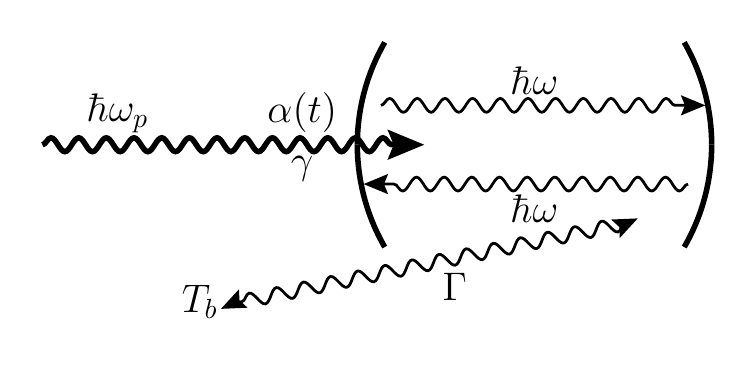
\begin{tikzpicture}[background rectangle/.style={fill=white}, show background rectangle]
% bounding box
% environment Box
%laser
\draw [line width = 2, decorate, decoration={snake}, -](0, 0) -- node [above left] {\Large $\hbar\omega_p$} (3, 0) -- node [above] {\Large $\alpha(t)$} node [below] {\Large $\gamma$} (3.6, 0) -- (4.5, 0);

\path (2, -2) node {\Large $T_b$};

% OPO
\def\rad{2.6}
\draw [line width = 2] (4, 0) arc (180:150:\rad);
\draw [line width = 2] (4, 0) arc (180:210:\rad);
\draw [line width = 2] (8.5, 0) arc (0:30:\rad);
\draw [line width = 2] (8.5, 0) arc (0:-30:\rad);

% light in OPO
\draw [line width = 1, decorate, decoration={snake}, -](4.3, 0.5)--
  node [above] {\Large $\hbar\omega$}(8.2, 0.5);
\draw [line width = 1, decorate, decoration={snake}, -](8.2, -0.5)--
  node [below] {\Large $\hbar\omega$}(4.3, -0.5);

% loss
\draw [line width = 1, decorate, decoration={snake}, -](7.4, -1)--
  node [below right] {\Large $\Gamma$}(2.5, -2);

% arrowheads
\path (4.55, 0) node [dart, fill=black, scale=0.75] {};
\path (8.22, 0.5) node [dart, fill=black, scale=0.5] {};
\path (4.28, -0.5) node [dart, fill=black, scale=0.5, shape border rotate=180] {};
\path (7.38, -1.02) node [dart, fill=black, scale=0.5, rotate=25] {};
\path (2.45, -2) node [dart, fill=black, scale=0.5, rotate=-155] {};
\end{tikzpicture}

\end{document}